\section{StreamIt}
\label{sec:streamit}

StreamIt  is   an  architecture-independent  language that was
designed for  streaming applications. In StreamIt, programs are
represented as graphs where  nodes represent  computation and edges
represent FIFO-ordered communication of data over tapes.

The  basic programmable  unit (i.e., an actor) in  StreamIt is a {\it
filter}.   Each filter contains  a work  function that executes
atomically,  popping (i.e., reading)  a fixed number  of items  from
the  filter's input  tape and pushing (i.e., writing) a fixed number
of items to the filter's output tape.  A filter  may also {\tt peek} at
a given index  on its input tape without  consuming  the  item;  this
makes  it  simple  to  represent computation over a
sliding-window.   The {\tt push}, {\tt pop}, and {\tt peek} rates are
declared as part  of  the work  function,  thereby enabling  the
compiler    to construct a static schedule of filter executions. The
following is an example implementation of a FIR   (Finite Impulse
Response)  filter: 
%\begin{scriptsize}
{\small
\begin{verbatim}
float->float filter FIR (int N, float[] weights) 
{
  work push 1 pop 1 peek N {
    float sum = 0;
    for (int i = 0; i < N; i++) {
      sum += peek(i) * weights[i];
    }
    pop();
    push(sum);
  }
}
\end{verbatim}}
%\end{scriptsize}

The work function is invoked (fired) whenever there is sufficient data
on the input tape. In this case, the filter requires at least
\texttt{N} elements before it can execute. The value of \texttt{N} is
known at compile time when the filter is composed to form a stream
graph. A filter is akin to a class in object oriented programming
with the work function serving as the main method. The parameters
to a filter (e.g., \texttt{N} and \texttt{weights}) are equivalent to
parameters passed to a class constructor. In StreamIt, the
application developer focuses on the hierarchical assembly of the
stream graph and its communication topology, rather than on the 
explicit management of the data buffers between filters.

\begin{figure}[t]
\begin{center}
\vspace{-12pt}
 \framebox{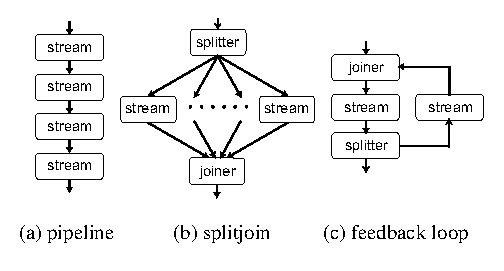
\includegraphics[scale=1, angle=0]{./constructs-eg.eps}}
 \caption{StreamIt containers.}
 \label{fig:containers}
\end{center}
\end{figure}

\begin{figure}[t]
\begin{center}
\vspace{-12pt}
 \framebox{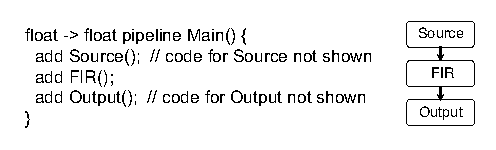
\includegraphics[scale=1, angle=0]{./pipeline-eg.eps}}
 \caption{Example pipeline with FIR filter.}
 \label{fig:pipeline}
\vspace{-24pt}
\end{center}
\end{figure}

StreamIt provides three hierarchical structures for composing filters
into larger stream graphs (see Figure~\ref{fig:containers}). The 
{\it pipeline} construct composes streams in sequence, with the output
of one connected to the input of the next.   An example of a pipeline
appears in Figure~\ref{fig:pipeline}.

The {\it splitjoin} construct distributes data to a set of parallel
streams, which are then joined together in a round robin fashion.  In
a splitjoin, the {\it splitter} performs the data scattering, and the
{\it joiner} performs the gathering. A splitter is a specialized
filter with a single input and  multiple output channels. On 
every execution step, it can distribute its output to any one of
its children in either a {\it duplicate} or a {\it roundrobin}
manner. For the former, incoming data is replicated to every
sibling connected to the splitter. For the latter, data is scattered
in a round-robin manner, with each item sent to exactly one child
stream, in order.  The splitter type and the weights for distrubuting data to
child streams are declared as part of the syntax (e.g., \texttt{split
duplicate} or \texttt{split roundrobin($w_0$, $w_1$, ... $w_n$)}). The
splitter counterpart, the joiner, is a specialized filter with  
multiple input channels but only one output channel. The joiner
gathers data from its predecessors in a round-robin manner (declared
as part of the syntax). 

StreamIt also provides a {\it feedback loop} construct for introducing
cycles in the graph.

\section{Execution Model}
\label{sec:execmodel}

A StreamIt program is represented by a hierarchical graph,
where the leaf nodes are filters, splitters, and joiners, and
the composite nodes are pipelines, splitjoins, and
feedback-loops. Edges in the graph represent data channels, which 
operate as FIFO queues.
In order for an actor  (i.e., a filter,
splitter, or joiner) to execute, it must have enough data items on its input
tape. In StreamIt, actors have  two epochs
of execution: one for initialization, and one for the steady
state. The initialization primes the input tapes to allow filters with
peeking to execute the very first instance of their work functions;
initialization in this setting is similar to the prologue stage in
software pipelining. The steady state schedule has the property that
the amount of data buffered between any two actors does not change
before and after the actor executions.

\begin{figure}[t]
\begin{center}
\vspace{-12pt}
 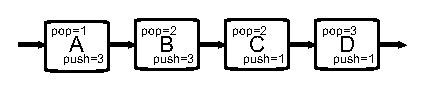
\includegraphics[scale=1, angle=0]{./pipe-with-rates.eps}
\vspace{-6pt}
 \caption{Example pipeline.}
 \label{fig:pipe-with-rates}
\end{center}
\end{figure}

As an example, a steady state schedule for the sample pipeline in
Figure~\ref{fig:pipe-with-rates} requires filter \texttt{A} to fire
four times, \texttt{B} six times, \texttt{C} nine times, and
\texttt{D} three times. 
% Because in StreamIt the filters are
% independent (i.e., they do not share state), they can execute
% concurently. In a uniprocessor setting (which is what we use for our
% evaluation), we can only run one filter at time. Therefore, 
The data generated by one actor is buffered (cached) until it is
comsumed.

The StreamIt compler derives the initialization and steady state
schedules~\cite{karczma-lctes03} and outputs a C program that includes
the initialization and work functions, as well as a driver to execute
each of the two schedules. For example, referring to
Figure~\ref{fig:pipe-with-rates}, the compiler generates the following
sample code for running the steady state schedule:
%\begin{scriptsize}
\begin{verbatim}
run_steady_state() {
  for (i = 0; i < 4; i++) A_work();
  for (i = 0; i < 6; i++) B_work();
  for (i = 0; i < 9; i++) C_work();
  for (i = 0; i < 3; i++) D_work();
}
\end{verbatim}
%\end{scriptsize}
To execute the program, the steady state kernel is wrapped with
another loop that invokes the kernel a designated number of
times. Preceeding the state steady, a similar initialization schedule
is run to prime the data buffers, and following the steady state, an
epilogue is run to drain the buffers as necessary.

\begin{figure}[t]
\begin{center}
\vspace{-12pt}
 \psfig{figure=ssi.eps,width=3in}
 \caption{Instruction size (in bytes along the y-axis) per filter
 (x-axis) occuring in a steady state execution of FFT.}
 \label{fig:ssi-single}
\vspace{-24pt}
\end{center}
\end{figure}

From a caching point of view, it is intuitively clear that once a
filter's instruction working set is fetched into the cache, we must
excute that filter as many times as possible to improve instruction
locality and amoritize the cost of the accesses to lower levels of the
memory hierarchy. This of course assumes that the total code size for
the filters in the steady state exceeds the capacity of the
instruction cache (which is commonly the case;). In
Figure~\ref{fig:ssi-single} we show a representative breakdown of the
code size per filter in a steady state execution of a StreamIt
implementation of FFT. In all, the total code size for a steady state
ranges from 16~Kb to over 60~Kb for our benchmarks. These results
provide evidence that while individual filters may have a
small instruction footprint, the total footprint of the filters in a
steady state exceeds a typical instruction cache size.
From these observations, it is evident that we must {\it scale} the
execution of filters in the steady state in order to improve temporal
locality. In other words, rather than running a filter $S$ times per
steady state, we increase the loop bound so that it runs $\texttt{M}
\times S$ times (e.g., the loop bound for \verb+A_work+ is
changed to $\texttt{M} \times 4$ in the example shown earlier). 
We term \texttt{M} the {\it multiplicity factor}.

The obvious question is: to what extent can we scale the execution of
filters in the steady state? The answer is non-trivial because
scaling, while beneficial to the instruction cache behavior, may
overburden the data cache as the buffers between actors may grow to
prohibitively large sizes that degrade the data cache
behavior. Specifically, if a buffer overflows the cache, then
produce-consumer locality is lost. 

Also complicating matters is the amount of state a filter must retain
from one execution of its work function to the next. In the FIR
example shown earlier, the filter state is proportional to the size of
the coeffecient array (i.e., \texttt{weights}). The filter state
further constrains the schedule scaling.
